\frameT{Outline}{
  \begin{enumerate}
    {\transparent{0.2} \item The languages of P-trees, PLP-trees, and LP-trees}
    \item Learning of preference models (PLP-trees and P-forests)
    {\transparent{0.2} \item Reasoning with preferences:
      \begin{itemize}
        \item Computing winners and ``strong" outcomes when votes are LP-trees
        \item Application in trip planning
      \end{itemize}}
    {\transparent{0.2} \item Future research directions}
  \end{enumerate}
}

\frameT{Learning Problems on PLP-trees}{
	\begin{block}{Consistent Learning (\tsc{ConsLearn})}
		Given an example set $\cE$, decide 
		whether there exists a PLP-tree $T$ (of a particular type) such that $T$ 
		is consistent with $\cE$.
	\end{block}

	\begin{block}{Small Learning (\tsc{SmallLearn})}
		Given an example set $\cE$
		and a positive integer $l$ ($l \leq |\cE|$), decide whether there 
		exists a PLP-tree $T$ (of a particular type) such that $T$ is consistent 
		with $\cE$ and $|T| \leq l$.
	\end{block}

	\begin{block}{Maixmal Learning (\tsc{MaxLearn})}
		Given an example set $\cE$ and a 
		positive integer $k$ ($k \leq m$), decide whether there exists a PLP-tree 
		$T$ (of a particular type) such that $T$ satisfies at least $k$ examples 
		in $\cE$.
	\end{block}
}

\frameT{Complexity Results on PLP-trees} {
  \begin{figure}[!ht]
    \centering
    \begin{subfigure}[b]{0.45\textwidth}
      \centering
      \begin{tabular}[0.45\textwidth]{ | c | c | c | }
        \hline
           & UP & CP \\
        \hline
        UI & P & P\\
        \hline
        CI & NPC\footnotemark & P  \\
        \hline
      \end{tabular}
      \caption{\tsc{ConsLearn}}
    \end{subfigure}
      \footnotetext{\scriptsize Booth et al., \tit{Learning Conditionally Lexicographic
            Preference Relations}, 2010.}
    \begin{subfigure}[b]{0.45\textwidth}
      \centering
      \begin{tabular}[0.45\textwidth]{ | c | c | c | }
        \hline
           & UP & CP \\
        \hline
        UI & NPC & NPC \\
        \hline
        CI & NPC & NPC \\
        \hline
      \end{tabular}
      \caption{\tsc{SmallLearn}}
    \end{subfigure} \\
    \begin{subfigure}[b]{0.45\textwidth}
      \centering
      \begin{tabular}[0.45\textwidth]{ | c | c | c | }
        \hline
           & UP & CP \\
        \hline
        UI & NPC\footnotemark & NPC \\
        \hline
        CI & NPC & NPC \\
        \hline
      \end{tabular}
      \caption{\tsc{MaxLearn}}
    \end{subfigure}
    \caption{Complexity results for passive learning problems}
  \end{figure}
  \footnotetext{\scriptsize Schmitt and Martignon, \tit{On the Complexity of
            Learning Lexicographic Strategies}, 2006.}
}

\frameT{Experimental Results on PLP-trees}{
  \begin{figure}[ht!]
    \centering
      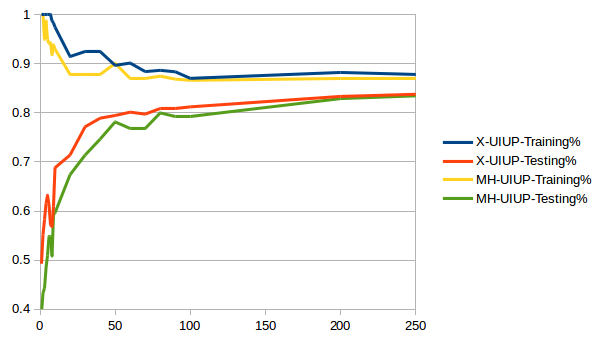
\includegraphics[width=0.7\textwidth]{figs/PrefLearnResults/Trees/X_MH/CarEvaluation.png}
    \caption{Learning curve for UIUP using ASP and greedy heuristic}
  \end{figure}
}

\frameT{Experimental Results on PLP-trees}{
  \begin{figure}[ht!]
    \centering
      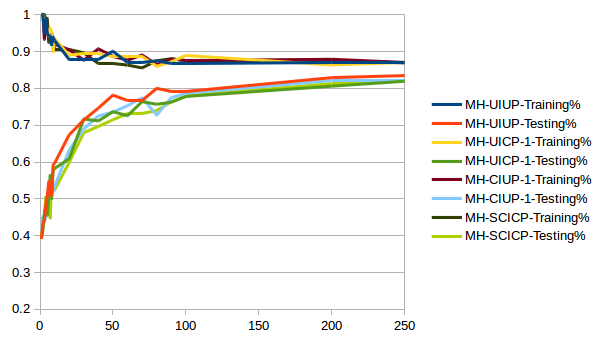
\includegraphics[width=0.7\textwidth]{figs/PrefLearnResults/Trees/MH/CarEvaluation.png}
    \caption{Learning curve for all four classes using greedy heuristic}
  \end{figure}
}

%\frameT{Preference Forests (P-Forests)}{
%	\begin{enumerate}
%		\item A \tit{preference forest} $F$ is a collection of PLP-trees
%					$F = \{T_1,\ldots,T_n\}$.
%		\item Denote by $N_F(o_1,o_2)=|\{T \in F:o_1 \succ_T o_2\}|$.
%		\item Given a preference forest $F$, and two outcomes $o_1$ and $o_2$, 
%					we say that $o_1 \succ_F^\Maj o_2$ iff $N_F(o_1,o_2)>N_F(o_2,o_1)$,
%					and that $o_1 \approx_F^\Maj o_2$ iff $N_F(o_1,o_2)=N_F(o_2,o_1)$.
%		\begin{itemize}
%			\item Pro: intuitive, decided in polynomial time.
%			\item Con: Condorcet paradox.
%			\item Other aggregating rules: positional scoring rules, Copeland's method, etc.
%		\end{itemize}
%	\end{enumerate}
%}
%
%\frameT{Experimental Results on P-Forests}{
%  \begin{figure}[ht!]
%    \centering
%      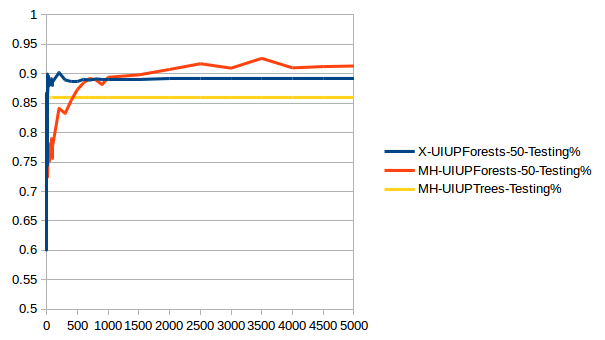
\includegraphics[width=0.7\textwidth]{figs/PrefLearnResults/Forests/X_MH/CarEvaluation.png}
%    \caption{Learning UIUP using ASP and greedy heuristic}
%  \end{figure}
%}
%
%\frameT{Experimental Results on P-Forests}{
%  \begin{figure}[ht!]
%    \centering
%      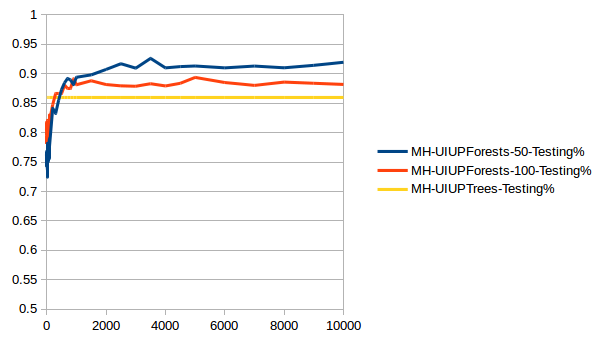
\includegraphics[width=0.7\textwidth]{figs/PrefLearnResults/Forests/MH/CarEvaluation.png}
%    \caption{Learning all four classes using greedy heuristic}
%  \end{figure}
%}
